\autobookmark
\begin{frame}[t]{Restarting the simulation to counter high MSE values}
      \myonly{1}{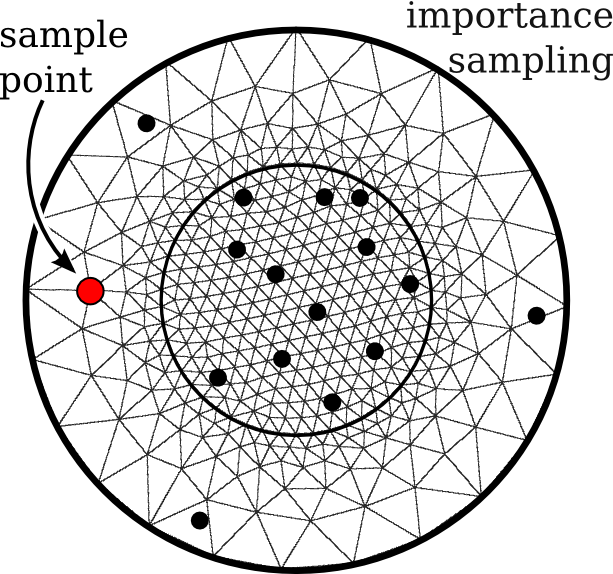
\includegraphics[width=.37\paperwidth]{graphics/ray_distributions3.png}}
      \myonly{2}{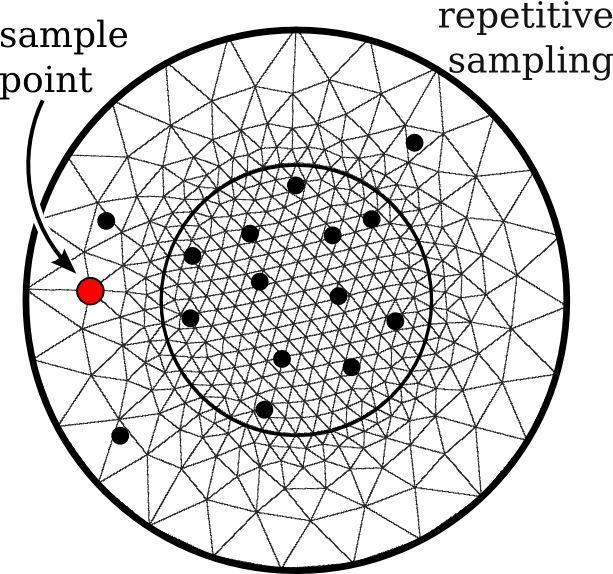
\includegraphics[width=.37\paperwidth]{graphics/ray_distributions5.png}}
      \myonly{1}{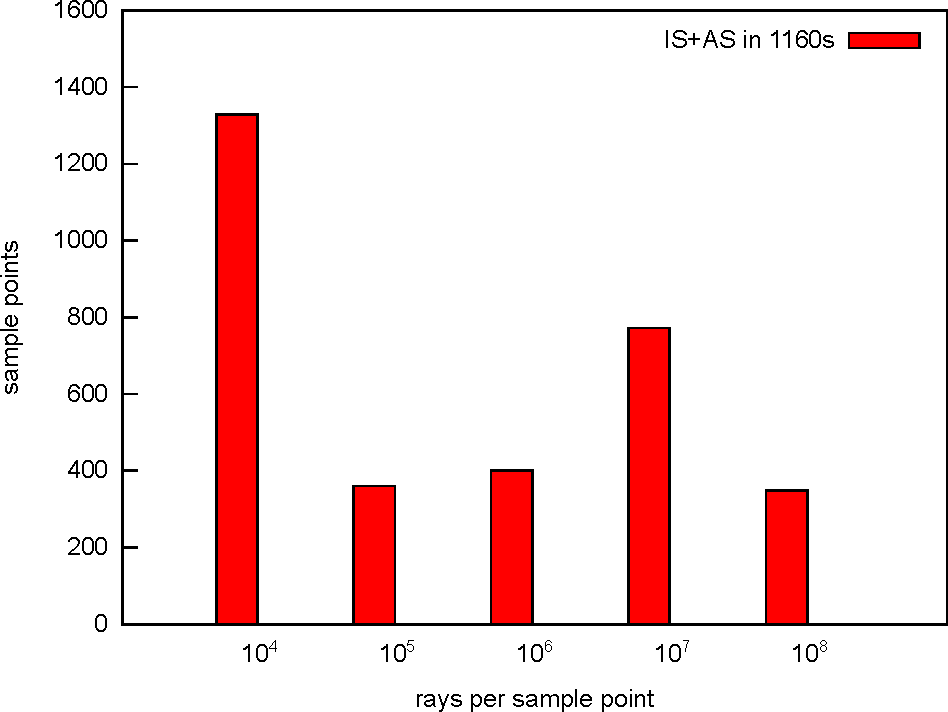
\includegraphics[width=.45\paperwidth]{graphics/mse_histogram_rs1.pdf}}
      \myonly{2}{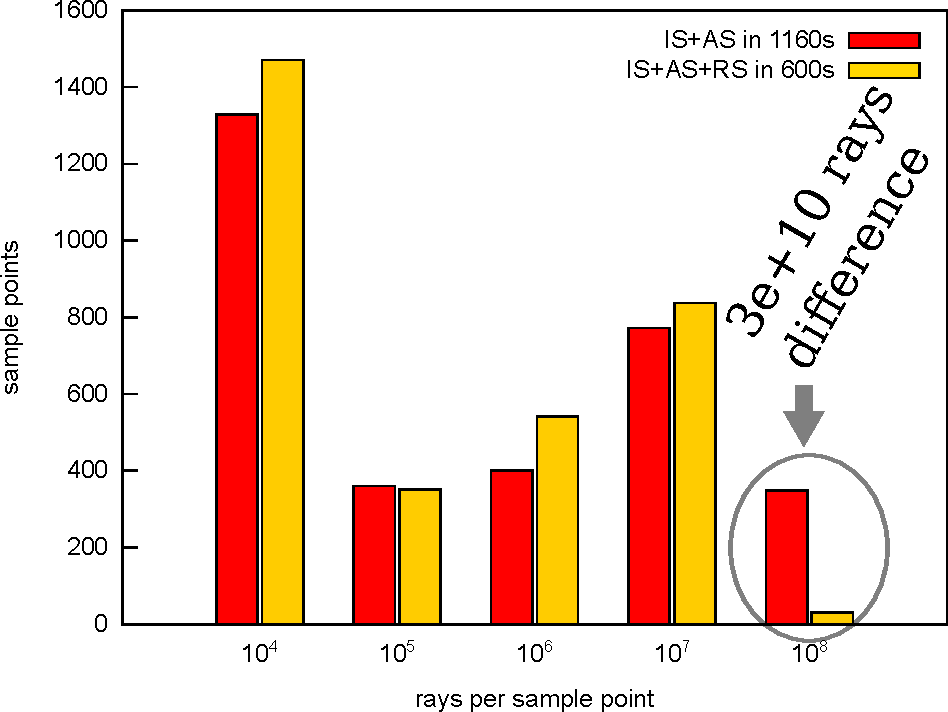
\includegraphics[width=.45\paperwidth]{graphics/mse_histogram_rs2.pdf}}
      \begin{itemize}
          \myuncover{1}{2}{
          \item Sometimes, increasing the number of rays is not necessary, because the high MSE was caused by a really unlucky seed for the PRNG
          }
          \myuncover{2}{2}{
          \item Idea: it might be enough to introduce random restarts, since this is much faster than increasing the number of rays
          }
      \end{itemize}


\end{frame}

%\begin{frame}{Predefined colours}
%  The template defines a set of colours according to the CD guidelines:\par
%  \begin{itemize}
%      \begin{minipage}[t]{0.5\linewidth}
%      \item \textcolor{hzdr-blue}{Helmholtz Blue}    
%      \item \textcolor{hzdr-orange}{Rossendorf Orange}  
%      \item \textcolor{hzdr-darkblue}{Helmholtz Dark Blue}
%      \item \textcolor{hzdr-gray1}{Gray1}   
%      \item \textcolor{hzdr-gray2}{Gray2}   
%      \item \textcolor{hzdr-gray3}{Gray3}   
%      \item \textcolor{hzdr-struct}{Structure of Matter}  
%      \end{minipage}%
%      \begin{minipage}[t]{0.5\linewidth}
%      \item \textcolor{hzdr-health}{Health}  
%      \item \textcolor{hzdr-energy}{Energy}  
%      \item \textcolor{hzdr-earth}{Earth and Environment}   
%      \item \textcolor{hzdr-keytec}{Key Technologies}  
%      \item \textcolor{hzdr-aero}{Aeronautics, Space and Transport}
%      \end{minipage}
%  \end{itemize}
%\end{frame}

